\chapter{Technique Overview}\label{ch:research}
This part of the thesis constitutes the main part.
The objective is to create an overview of techniques in the field which may be used to solve the
problem detailed in Chapter~\ref{ch:problem}.
First the search for literature which lays the foundation for the subsequent sections, is documented.
The a taxonomy is introduced which facilitates the analysis and comparison of techniques.
Lastly, the advances in the field are placed in the correct position and analyzed.

\section{Taxonomy of Pipeline Steps}
In order to create the overview the necessary steps in the process of \ac{STS} need to be highlighted,
from preprocessing to classifying the identified text~\citep{long_scene_2021, sourvanos_challenges_2018}.
The ways in which the respective issues for the steps are solved are identified from literature,
listed and explained alongside.
\begin{figure}[h]
    \centering
    \resizebox{\linewidth}{!}{
\begin{tikzpicture}[
    every node/.style={draw=black,thin,anchor=west, minimum height=2.5em},
    lroot/.style={%
        edge from parent fork down,
        level distance=0.5cm,
        text centered, text width=3cm},
    lone/.style={%
        text centered, text width=3cm,
        level distance=0.5cm},
    ltwo/.style={%
        text centered, text width=3cm,
        level distance=0.5cm},
    lthree/.style={%
        rounded corners,
        grow=down, xshift=-0.8cm,
        text centered, text width=3cm,
        edge from parent path={(\tikzparentnode.205) |- (\tikzchildnode.west)}},
    level1/.style ={level distance=1.2cm},
    level2/.style ={level distance=2.4cm},
    level3/.style ={level distance=3.6cm},
    level4/.style ={level distance=4.8cm},
    level5/.style ={level distance=6.0cm},
    level 1/.style={sibling distance=8cm},
    level 1/.append style={level distance=1.5cm},
    level 2/.style={sibling distance=4cm},
    level 2/.append style={level distance=1.5cm},
]
%   \draw[help lines] (0,0) grid (4,3);

    % lroot
    \node[anchor=south,lroot]{STS}
    [edge from parent fork down]
        child{node [lone] {STD}
            child{node [ltwo] {Regressor \\ based}
                child[lthree,level1] {node {Feature \\ Extraction}}
                child[lthree,level2] {node {BB \\ Regresseion}}
                child[lthree,level3] {node {IOU \\ matching}}
            }
            child{node [ltwo] {Segmentation \\ based}
                child[lthree,level1] {node {Sub-components \\ segmentation}}
                child[lthree,level2] {node {Text \\ reconstruction}}
            }
        }
        %
        child{node [lone] {STR}
            child{node [ltwo] {Regressor \\ based}
                child[lthree,level1] {node {Image \\ preprocessing}}
                child[lthree,level2] {node {Character \\ segmentation}}
                child[lthree,level3] {node {Character \\ recognition}}
            }
            child{node [ltwo] {Segmentation \\ based}
                child[lthree,level1] {node {Image \\ preprocessing}}
                child[lthree,level2] {node {Feature \\ extraction}}
                child[lthree,level3] {node {Sequence \\ modelling}}
                child[lthree,level4] {node {Prediction}}
            }
        }
        %
        child{node [lone] {E2E}
            child{node [ltwo] {Two Stage}
                child[lthree,level1] {node {STD}}
                child[lthree,level2] {node {STR with \\ feature maps}}
            }
            child{node [ltwo] {One Stage}
                child[lthree,level1] {node {STD \& STR \\ Parallel}}
            }
        };

\end{tikzpicture}
}%


\begin{comment}
\begin{tikzpicture}[
    font=\scriptsize,
    edge from parent fork down,
    level distance=1.75cm,
    every node/.style={
            rectangle,
            minimum height=6mm,
            align=center,
            text depth = 0pt,
    },
    edge from parent/.style={draw=black},
    category/.style={Rectangle},
    step/.style={Circle}
]
    \Tree [.STS
        [.{STD}
            [.{Feature \\ Extraction} ]
            [.{BB Regression} ]
        ]
        [.{STR}
            [.{Preprocessing} ]
            [.{Feature \\ Extraction} ]
            [.{Sequence \\ Modelling} ]
            [.{Prediction} ]
        ]
    ]
\end{tikzpicture}
\end{comment}

\caption{Pipeline taxonomy and respective steps\label{fig:pipelineSteps}}
\end{figure}
Figure~\ref{fig:pipelineSteps} shows tasks which are associated with \ac{STS}.
\ac{STD} and \ac{STR} only incorporate a part of \ac{STS}, while E2E
incorporate both \ac{STD} and \ac{STR} techniques to solve \ac{STS}~\citep{long_scene_2021}.
Therefore this section will first discuss the two parts, to then combine them.

For \ac{STD} two main categories of approaches can be identified: segmentation based and segmentation
free~\citep{long_scene_2021,sheng_centripetaltext_2021,liu_accurate_2020}.
The segmentation free category draws heavy inspiration from the field of object
detection~\citep{long_scene_2021,liu_accurate_2020}.
This is only natural as text detection can be seen as a type of object
detection~\citep{liu_accurate_2020,long_scene_2021}.
For object detection inspired \ac{STD} there are mainly two methods: one stage i.e.\ anchor based
and two stage i.e. \ac{ROI} based~\citep{long_scene_2021}.
Both localize text instances as a whole~\citep{long_scene_2021,sheng_centripetaltext_2021}.
One stage or anchor based approaches are modelled after~\cite{liu_ssd_2016} (Single Shot MultiBox
Detector --- SSD) and~\cite{redmon_you_2016} (You Only Look Once --- YOLO).
\begin{figure}[ht]
    \centering
    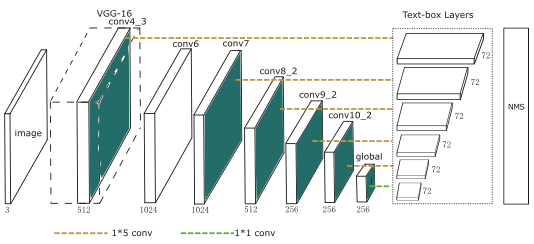
\includegraphics[width=0.8\textwidth]{img/STD-seg-free-Liao-TextBoxes-2017.png}
    \caption{Example for an anchor based, segmentation free STD
    architecture~\citep{liao_textboxes_2017}\label{fig:STD-segfree}}
\end{figure}
The basic approach is explained with the example of~\cite{liao_textboxes_2017} which is based on
SSD (see Figure~\ref{fig:STD-segfree}).
It uses 13 layer convolutional network (three blocks of: two or three $3\times3$ conv layers followed
by a $2\times2$ max pooling layer) for feature extraction~\citep{liao_textboxes_2017}.
Afterwards come nine additional layers which continuously downsample, the output of six of them
is separately used as feature maps for \ac{BB} regression~\citep{liao_textboxes_2017}.
% FIXME: source?
The downsampling and \ac{BB} regression for different layers helps detect text instances of different
sizes.
%
The \ac{BB} regression is carried out by six text-box layers which predict how probable a text
instance (c) is in the respective area and predict where the text instance is ($x,y,w,h$).
These layers are the difference to the SSD approach for normal object
detection~\citep{liao_textboxes_2017,liu_ssd_2016}.
Note that the output is not the location of a \ac{BB} but the offset to the
respective anchor box~\citep{liao_textboxes_2017}.
Anchor boxes are predefined to give bias towards sizes and aspect ratios of
text~\citep{liao_textboxes_2017}.
Additionally, the text-box layers use $1\times5$ filters to adjust to larger aspect
ratios~\citep{liao_textboxes_2017}.
Each text-box layer has 72 filters (12 anchor boxes $\cdot$ 6 values per prediction), the filters
are slided accross the input features generating 12 predicted \ac{BB} per
position~\citep{liao_textboxes_2017}.
The \acp{BB} of all layers are then subjected to the process of \ac{NMS} to filter out the best
\ac{BB} for each possible text instance~\citep{liao_textboxes_2017}.
%FIXME: umschreiben: erst SSD erklären und dann veränderung für STD?

% FIXME: ROI methods
The R-CNN which builds the foundation for \ac{ROI} based text detection, was introduced
by~\cite{girshick_rich_2014} and improved by~\cite{girshick_fast_2015} (Fast
R-CNN),~\cite{ren_faster_2015} (Faster R-CNN) and~\cite{he_mask_2018} (Mask R-CNN).
The model introduced by~\cite{jiang_r2cnn_2017} uses Faster R-CNN.

STD
\begin{itemize}
    \item ROI proposal (two stage): feature extraction, ROI proposal, ROI pooling
            (like R-CNN)
    \item segmentation based: segment text areas (different granularity: pixel, component,
        character), assemble text instances (reconstruction)
\end{itemize}

STR
\begin{itemize}
    \item segmentation-free approach (segmentation-based implicit and explicit out of date)
    \item Steps: Preprocessing, Feature Extraction, Sequence Modelling, Prediction
    \item preprocessing, text enhancement: remove distortions, background; improve resolution,
        recover degraded text
        \begin{itemize}
            \item Spatial Transformer Networks (for distortions)
        \end{itemize}
    \item feature extraction: encode image into feature space
        \begin{itemize}
            \item ResNet
                \begin{itemize}
                    \item aggressive downsampling
                    \item $3\times3$ best kernel size
                    \item Gradient saving $\rightarrow$ Res block, Res Bottleneck, Res Grouped
                    \item batch normalization
                    \item 32,50,150,\ldots
                \end{itemize}
            \item GoogLeNet
        \end{itemize}
    \item Sequence and Prediction
        \begin{itemize}
            \item CTC
            \item Encode-Decoder/Attention
            \item Lexicon Free Models!
        \end{itemize}
\end{itemize}

E2E
\begin{itemize}
    \item trainable as one?
    \item Bestandteile nicht zwangsweise sequentiell
    \item two step or two stage pipeline
\end{itemize}

\begin{comment}
What is segmentation
- Detection: from pixel to character -> better for arbitrary shapes
    - Segmentation
    - Text detection of of segmentation
- Recognition: are not used often (poor word-level results)
    - Segmentation
    - recognition
- End to end?
\end{comment}

\begin{figure}[ht]
    \centering
    \subfigure[Residual block~\citep{he_deep_2015}\label{fig:residual-block}]{%
        {\scriptsize%
\begin{tikzpicture}[scale=0.6]
    \node (l1) {conv 1};
    \node[right=4mm of l1, label={below:}] (act1) {$\relu$};
    \node[right=4mm of act1] (l2) {conv 2};
    \node[right=4mm of l2,font=\small,label={below:},inner sep=0,pin={60:$F(\X) + \X$}] (add) {$\oplus$};
    \node[right=4mm of add, label={below:}] (act2) {$\relu$};

    \draw[->] (l1) -- (act1);
    \draw[->] (act1) -- (l2);
    \draw[<-] (l1) -- ++(-2,0) node[below, pos=0.8] {$\X$};
    \draw[->] (l2) -- (act2) node[above, pos=0.8] {};
    \draw[->] ($(l1)-(1.5,0)$) to[out=30, in=150] node[below=1ex, midway, align=center]
        {} node[above, midway] {identity} (add);
    \draw[decorate, decoration={brace, amplitude=1ex, raise=1cm}] (l2.east) -- node[midway, below=1.2cm]
        {$F(\X)$} (l1.west);
\end{tikzpicture}
}
%
    }
    \subfigure[Residual block with pooling~\citep{ponti_everything_2017}\label{fig:residual-block}]{%
        {\scriptsize%
\begin{tikzpicture}[scale=0.6]
    \node (l1) {conv 1};
    \node[right=4mm of l1] (l15) {pooling};
    \node[right=4mm of l15, label={below:}] (act1) {$ReLU$};
    \node[right=4mm of act1] (l2) {conv 2};
    \node[right=4mm of l2,font=\Large,label={below:},inner sep=0,pin={90:$F(\X) + P(\X)$}] (add)
        {$\oplus$};
    \node[right=4mm of add, label={below:}] (act2) {$ReLU$};

    \draw[->] (l1) -- (l15);
    \draw[->] (l15) -- (act1);
    \draw[->] (act1) -- (l2);
    \draw[<-] (l1) -- ++(-2,0) node[below, pos=0.8] {$\X$};
    \draw[->] (l2) -- (act2) node[above, pos=0.8] {};
    \draw[->,dashed] ($(l1)-(1.5,0)$) to[out=30, in=150] node[below=1ex, midway, align=center]
        {$P(\X)$} node[above, midway] {pooling} (add);
    \draw[decorate, decoration={brace, amplitude=1ex, raise=1cm}] (l2.east) -- node[midway, below=1.2cm]
        {$F(\X)$} (l1.west);
\end{tikzpicture}
}
%
    }
    \subfigure[Residual bottleneck block~\citep{he_deep_2015}\label{fig:residual-block}]{%
        {\scriptsize%
\begin{tikzpicture}[scale=0.6]
    \node (l1) {conv 1, $1\times1$};
    \node[right=2mm of l1, label={below:}] (act1) {$ReLU$};
    \node[right=2mm of act1] (l15) {conv 2, $3\times3$};
    \node[right=2mm of l15, label={below:}] (act15) {$ReLU$};
    \node[right=2mm of act15] (l2) {conv 3, $1\times1$};
    \node[right=2mm of l2,font=\small,label={below:},inner sep=0,pin={60:$F(\X) + \X$}] (add) {$\oplus$};
    \node[right=2mm of add, label={below:}] (act2) {$ReLU$};

    \draw[->] (l1) -- (act1);
    \draw[->] (act1) -- (l15);
    \draw[->] (l15) -- (act15);
    \draw[->] (act15) -- (l2);
    \draw[<-] (l1) -- ++(-3,0) node[below, pos=0.8] {$\X$};
    \draw[->] (l2) -- (act2) node[above, pos=0.8] {};
    \draw[->] ($(l1)-(2.5,0)$) to[out=30, in=150] node[below=1ex, midway, align=center]
        {} node[above, midway] {identity} (add);
    \draw[decorate, decoration={brace, amplitude=1ex, raise=1cm}] (l2.east) -- node[midway, below=1.2cm]
        {$F(\X)$} (l1.west);
\end{tikzpicture}
}
%
    }
    \caption{Modules introduced with ResNet\label{fig:resnet}}
\end{figure}

\section{Literature Search}\label{se:litSearch}
This section documents the search for literature which provides the content for the subsequent
overview of innovation.
For this, important pipelines and notable advances along with their properties are researched,
analysed and presented.
The literature is identified through searching in the Google Scholar database.
The search is executed with keywords such as, but not only: Deep Learning, Text Detection,
Text Recognition, Text Spotting, Scene Text, Pipeline.
% FIXME: update keywords
A criterion for further examination is an appropriate amount of citations for the piece of literature
in question.
Additionally, literature is selected through citations for and by literature which has already been
identified as important.
All research after 2018 which pertains to extracting scene text is regarded as relevant.
Standard \ac{OCR} solutions may not hold validity in practice, as the image and text conditions can
vary in the defined problem~\citep{chen_text_2021}.
The delimination from Section~\ref{se:problem} of course holds for this chapter and only literature
which concerns advances for the \ac{DL} model architecture will be regarded as important for the
scope of this thesis.
This extends to the whole pipeline from preprocessing an image to the final result of the model.

% FIXME: hierarchical graphic with found papers
% FIXME: describe proceeding


\section{State of the Art Methods}

text enhancement:~\cite{chen_text_2021}
model pruning:~\cite{niu_26ms_2019}
integer inference:~\cite{ignatov_ai_2019}
